\begin{table}[htbp]
\centering
\caption{Persona Primária}
\label{tab:Table_persona1}
\small
\begin{tabular}{| m{0.25\textwidth} m{0.65\textwidth}|}
\hline \multicolumn{2}{|c|}{\textbf{Identidade}} \\ \hline
& \\

\begin{center} 
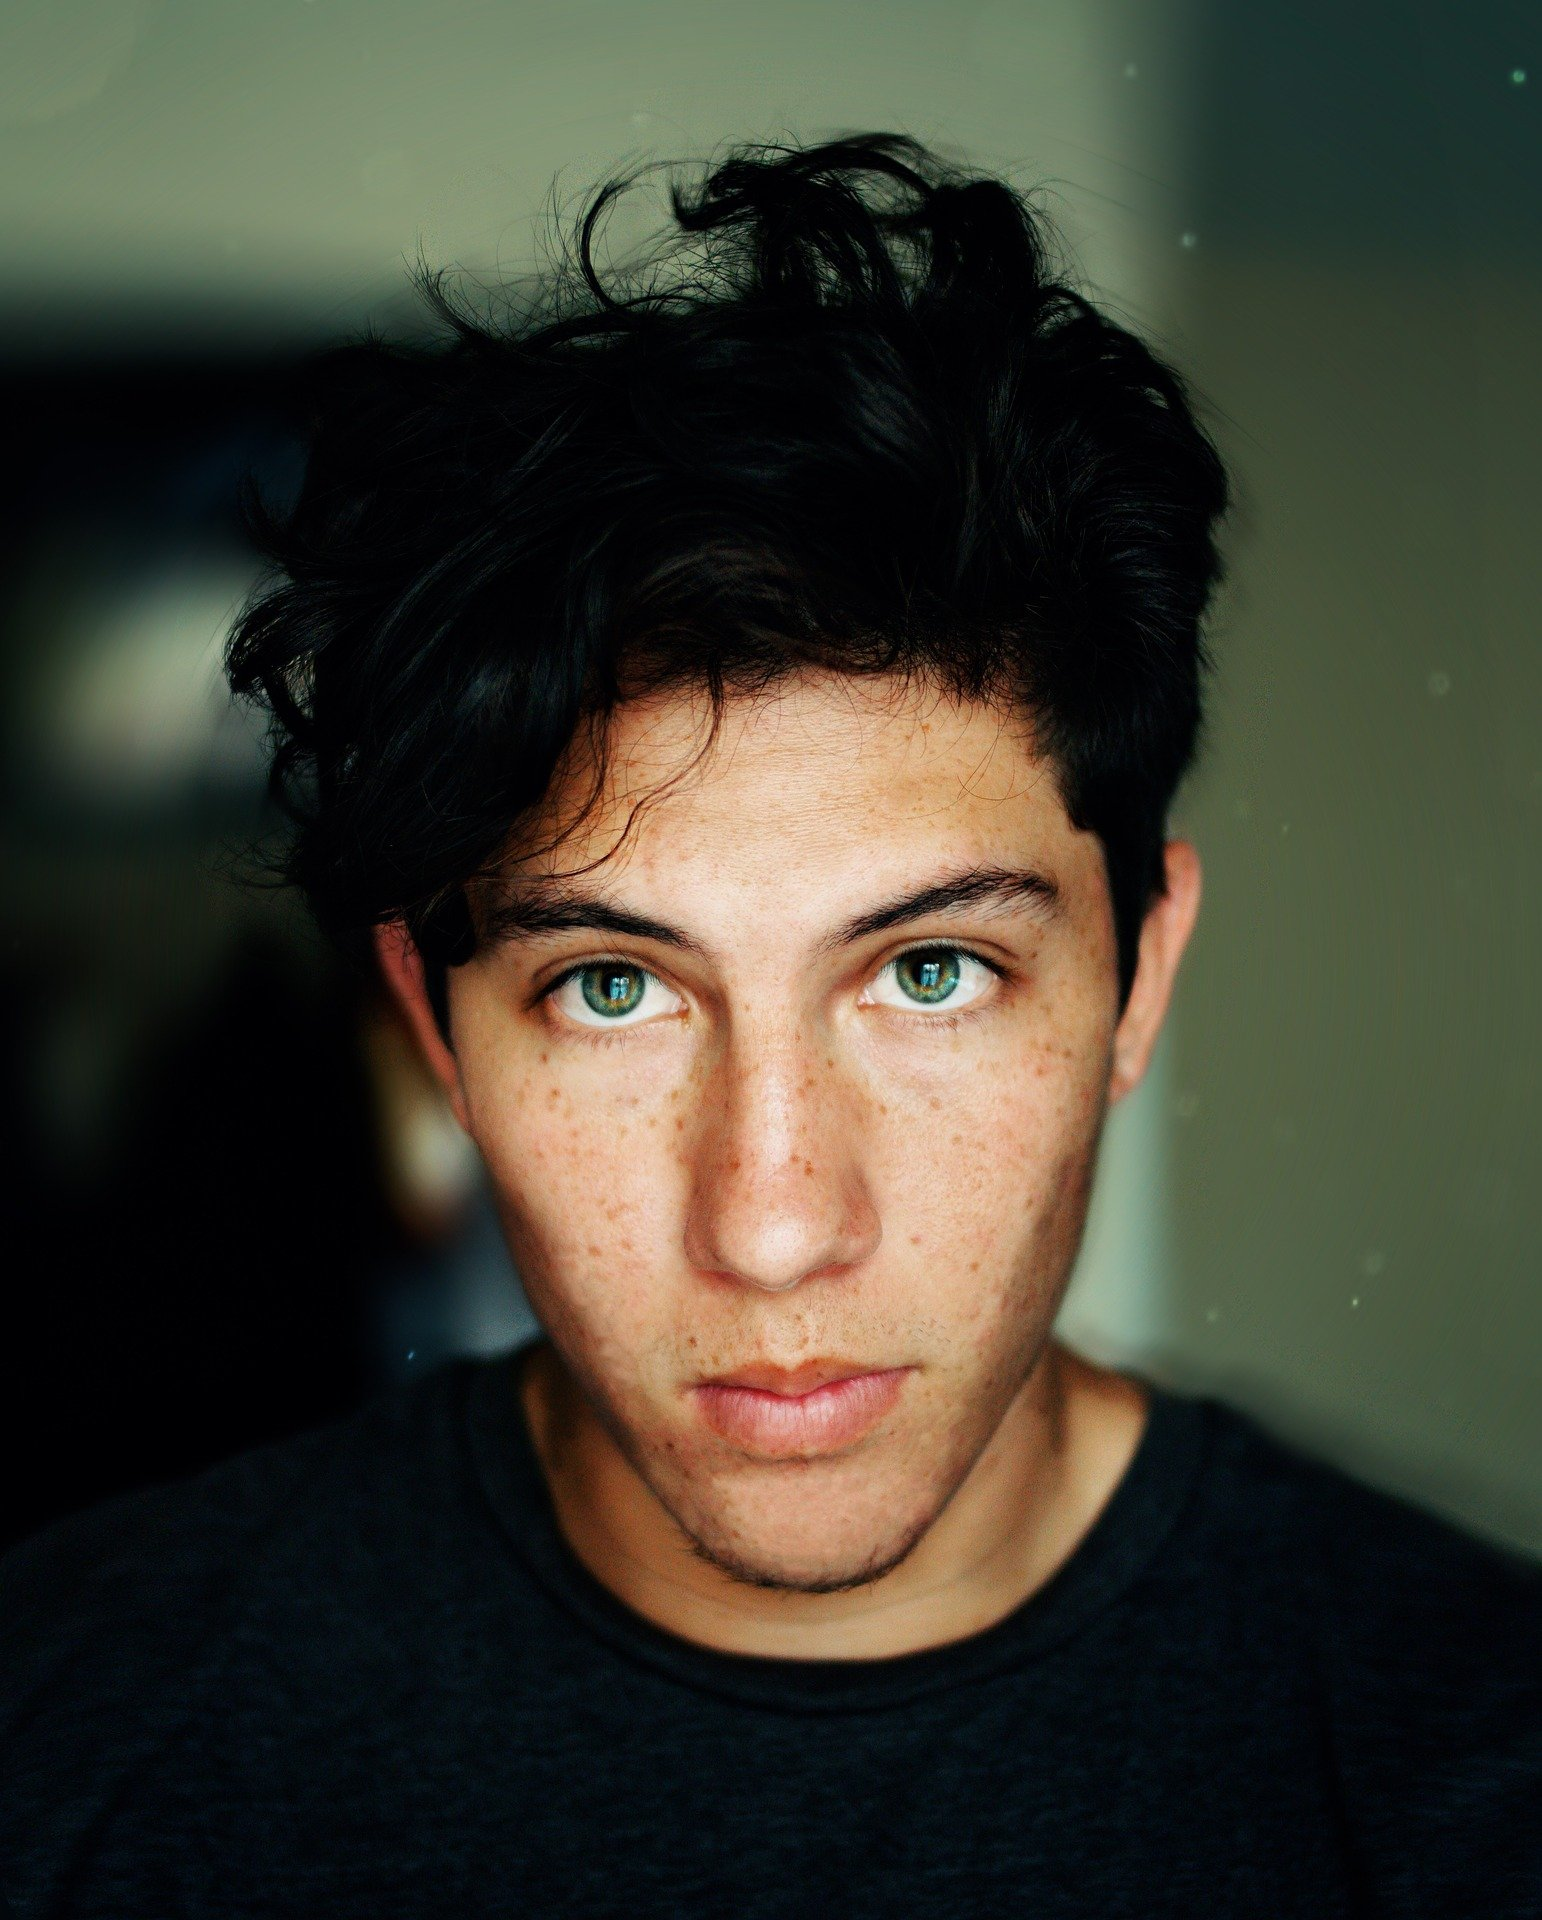
\includegraphics[scale=0.06]{figuras/personas/portrait-3353699_1920.jpg} 
Fonte: Pixabay\tablefootnote{https://pixabay.com/photos/portrait-people-adult-man-face-3353699/}
\end{center} 



&

\textbf{Nome: } Victor Matheus Farias

\textbf{Idade:} 19 anos

\textbf{Ocupação:} Estudante de Engenharia de Software na UnB, Faculdade do Gama.

\\ \hline


\multicolumn{2}{|c|}{\textbf{Descrição}} \\ \hline
\multicolumn{2}{|p{15cm}|}{
    \begin{tabular}[c]{@{}l@{}}\\
    Aprender um conteúdo novo é meu o principal objetivo ao usar jogos educacionais.\\ Atualmente eu uso alguns, mas com uma frequência moderada, não gosto de gastar\\ muito tempo com jogos. Vejo-os como ferramentas que me auxiliam no processo de \\aprendizagem. Estou cursando a disciplina de IHC e não tenho muito conhecimento \\em relação a elaboração de design de interfaces e o pouco que tenho está somente no \\âmbito disciplinar. Desejaria utilizar um jogo que me ajudasse a aprender o conteúdo.\\ 
    \\
    Geralmente quando vou estudar ou sanar alguma dúvida que tenho sobre o conteúdo \\eu pesquiso na internet, em alguns casos assisto vídeo aulas e também utilizo do \\material disponibilizado pelo professor.\\
    \\
    Um jogo educacional pra mim, deve \textbf{responder bem às minhas ações}, me ensinando\\ caso eu erre por exemplo; deve ter um \textbf{design legal}, talvez com um tema; deve ser \\\textbf{simples de se aprender a jogar}, não tendo regras extensas e tutorias longos; e \\também deve ser \textbf{fácil de jogar}. \\
    \\
    E por fim o que eu espero de um jogo educacional é sentir \textbf{satisfação}, aprender com um\\ pouco de \textbf{desafio} e \textbf{diversão} é muito bom. Ter a percepção da \textbf{relevância} do assunto\\ que estou aprendendo é algo que me dá \textbf{confiança} que vou atingir meu objetivo de\\ estudo. E mesmo não gostando de gastar muito tempo com jogos, mas se eu sentir que \\estou sendo produtivo com certeza vou me manter \textbf{focado}.\\ \\
    \end{tabular}
} \\ \hline
\end{tabular}
\end{table}
\newpage